
\section{Background}
\label{sec:background}

The current system of course selection, Webtree, was designed to allow
students to customize their course selections to deal with various
contingencies. For example, a student might want a different second
course option depending on whether or not he or she successfulling
recieved his or her first option. Webtree consists of three binary trees (depth
of $3$), which are traversed according to an elaborate
algorithm. Students' fourth class is ranked in order $1-4$, and is
selected according to availability in that order. For a visual
represention of Webtree, as well a chance to imagine the confusion that
many students feel when filling it out, see
Figure~\ref{fig:webtr}. Interested readers are referred to the
Davidson College Registrar's Office for a detailed description of the
Webtree algorithm\footnote{http://www.davidson.edu/offices/registrar/course-registration-and-webtree/how-to-use-webtree}.

\begin{figure}[htb]
  \centering  % centers the image in the column
  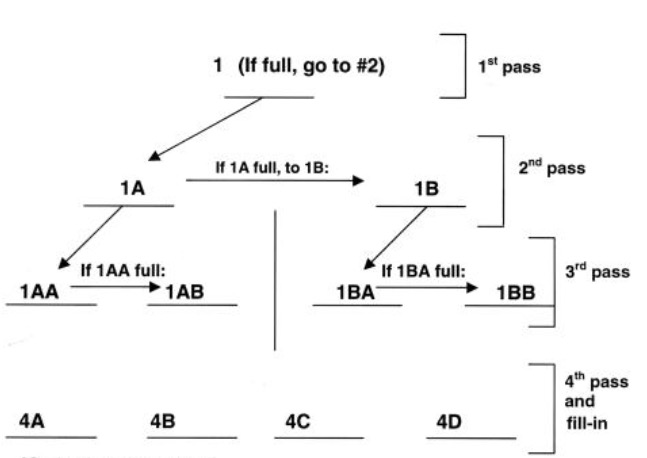
\includegraphics[width=0.37\textwidth]{figs/webtree.jpg}
  % *Every* figure should have a descriptive caption.
  \caption{The complicated nature of Davidson College's Webtree. Image
    courtesy of Davidson College Registrar.}
  \label{fig:webtr}
\end{figure}

Alternatively, we chose to approach this problem as a constraint
satisfaction problem. A constraint satisfaction problem takes the
inputs $Varibles$, $Domains$, and $Constraints$ \cite{aima}. We chose to
specifically implement this problem as a psuedoboolean constraint
satisfaction problem. A psuedoboolean problem has its domain limited
to {True, False}, or {0,1}. Thus, we set up our problem as a set of
constraints of inequalities, and an objective function that we attempt
to minimize. Several computer scientists have devoted time to creating
psuedoboolean solvers and allowing the public to have full access to
them.

To determine whether one method of scheduling is ``better'' than
another, we must devise a way of ranking a schedule. Since we are
given preferences in Webtree format, we must be able to assign an
individual request a certain rank. For our purposes, we have defined
rank of a scheduling assignment to be the sum of ranks of all the
courses assigned in that given assignment: \begin{equation}\label{rank}Rank_{scheduling} =
  \sum_{i=0}^{|Variables|}{rank(i)*x_i}\end{equation} 

A course is assigned a given rank depending on the tree and branch
that it was placed in the original Webtree. If a request was in the
first ``branch'' (i.e. the root node of a Tree), then the course is given
a rank {1-4}, according to which Tree it is in. For Trees {1-3}, the
rest of the courses are then ranked according to whether they are a
left child or a right child. Left children are a higher priority than right
children and given a rank of 1; right children are the second option
and thus given a rank of 2. Requests on Tree 4 are ranked {4-7}, in
the order that they are placed.



